\chapter{Developing Environment}

This section is aimed to present the development method as well as the programming language, tools, software and hardware used throughout the development of this bachelor thesis.

The section \ref{chapter3_methodology} introduces the methodology used for developing the kernel.

The section \ref{chapter3_software} introduces the different software and operating systems used in order to compile and use the kernel. In addition to that, the software used for the realisation of the project are also introduced. 


\section {Methodology}\label{chapter3_methodology}

The methodology used for developing the features of the operating system uses the TDD\footnote{Test-Driven Development}\cite{tdd} method. That is, when a feature is needed, a test is made and then the solution is developed. It helps to have a clear idea of the edge cases and what the function should do. Continuous automated testing of the projects offers several key advantages:
\begin{itemize}
\item\textbf{Documentation purposes:} Although it doesn't alone give a complete documentation of the function, it shows clearly how it should be used and why it has been thought for. The scenarios displayed in the tests should be typical scenario that can happen when using them in the project.
\item\textbf{Bug prevention:} A very common way to introduce bug in a library is to change the algorithm while keeping backward compatibility. If the feature has been tested, a developer shouldn't fear to update the internal implementation of a function (for example, improve the efficiency or enhance the results of said function) as the tests will fails if the function doesn't behave any more as it is expected to in at least one of the cases.
\item\textbf{Time saver:} Automated tests are very useful as they allows the developer to avoid testing every cases by hand when modifying a feature. The tests being automated, they will notify failures, if any, automatically. 
\end{itemize}

\begin{figure}
\begin{center}
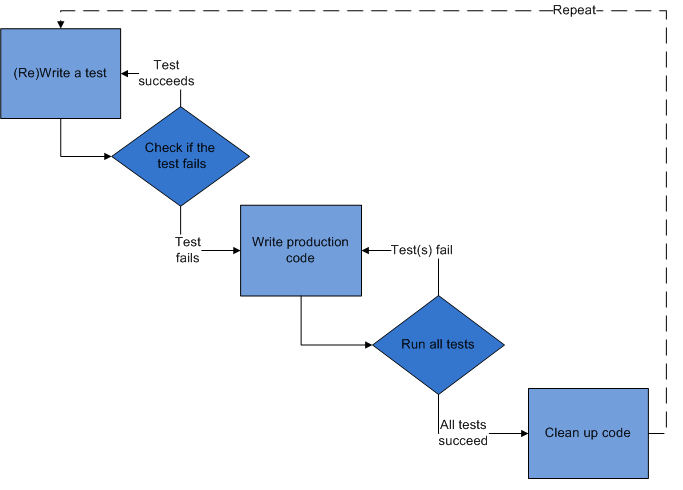
\includegraphics[width=0.5\textwidth]{includes/figures/chapter3_tdd_flowchart.png}  \\[0.5 cm]
\caption{Flowchart of a TDD-driven project}
\end{center}
\end{figure}


In this thesis, a tests have been created in any of these three scenarios:
\begin{itemize}
\item\textbf{Feature creation:} As stated by the TDD, a test should be created before implementing the solution.
\item\textbf{Feature enhancement:} If the algorithm has been changed and some behaviour has been modified, a test is created.
\item\textbf{Bug encountered:} When an unexpected scenario has been found leading to an incorrect behaviour, a test is created testing for the correct behaviour and then the function tested is modified to fit all the previously made tests as well as the newly created one.
\end{itemize}



\section{Software}\label{chapter3_software}

\subsection{Operating System}
The Operating System used for the development, compilation of the kernel and redaction of the documentation is Mac OSX version 10.10. This is the latest iteration of Apple's Operating System.


\subsection{Programming Language}

The end program needs to be compiled to an ARM assembly program, it is therefore all naturally that at the very beginning of the project, the kernel was implemented in ARM Assembly. However, as many people that wrote code in assembly know, assembly can reveal itself tedious to work with, I therefore looked for a way to use either the C or C++ programming languages. However, I've had way more practice with C, especially throughout the whole degree, than C++. It is very difficult to write the whole kernel without any ARM Assembly in it: The bootstrap of the kernel is written in ARM ASM (i.e.: The stack settings as well as the interrupt vector), and the higher level of code is written in C.

Regarding C, it is a general-purpose programming language created in 1972 by Dennis Ritchie and Brian Kernighan\cite{ritchie_c}, however, it is often used for low level programming or programs to be run from within a CLI\footnote{Command line interface}. It has been created to be mapped efficiently to machine code as an alternative to assembly programming, which is one of the main reasons why it is still nowadays a famous programming language for operating system development (Linux, for instance, is almost completely implemented in C).

Due to the popularity and the age of C, it proposed a wide range of advantage:
\begin{itemize}
\item Compatible with most current Operating System
\item Fast and efficient as it is really close to machine code
\item Lot of support and in our case, compiler and cross compilers for a large set of computers.
\item Modulable through the usage of libraries. 
\end{itemize}

As a drawback, C totally lacks of Object-Oriented features (C++ has been created to fix this issue), and it has a steep learning curve.


\subsection{Cross-Compiler}

A cross-compiler is a compiler that is able to create binary code for a machine different that on which the compiler is run. Since the code is not being compiled on the Raspberry Pi but instead, on independent computer, the use of a cross-compiler is mandatory.

In order to compile the kernel, the YAGARTO GNU ARM toolchain\cite{yagarto} has been used. The YAGARTO toolchain was initially made to be executable on Microsoft Windows with the objective to be independent from Cygwin\cite{cygwin}, a Unix-like environment and command-line interface for Microsoft Windows that provides native integration of Windows-based applications, data, and other system resources with applications, software tools, and data of the Unix-like environment. and be cheap for beginner (it is actually free). The YAGARTO project has then be ported to Mac OSX. Amongst other program, this toolchain comes with the following tools that are used for the compilation process:
\begin{itemize}
\item \textbf{arm-none-eabi-as:} Used for the compilation of the assembly code.
\item \textbf{arm-none-eabi-gcc:} Used for the compilation of the C code.
\item \textbf{arm-none-eabi-ld:} Used for the linking of the object files into an ELF\footnote{Executable Linkable Format} file following a given memory map.
\item \textbf{arm-none-eabi-objcopy:} Used to convert the compiled file back to assembly code, it is used mainly for debug purposes.
\end{itemize}


\subsection{Clang}

Clang is an open source compiler for the C, C++, Object-C and Objective C++ programming languages. It uses LLVM\footnote{Low Level Virtual Machine}\cite{llvm} as compiler infrastructure developed by Apple starting from 2007 but that has since then received involvement from other companies such as Google, ARM or even Intel. This is the compiler present by default on the Mac OSX operating system and the one used in this project to compile the code that can be executed by the users for the functional testings. 


\subsection{GNU Screen}

GNU Screen is a command-line application for console multiplexing, allowing a user to have different virtual consoles inside one terminal by the mean of different buffers. It has the particularity to able to be detached (i.e. put in the background) and restored later in time without pausing or closing the programs opened in screen. 
The most interesting feature and the one that is directly linked to this project is that GNU Screen can be used a serial console, that is, it is possible to specify a number of baud and a port so as to communicate with a peripheral. This is therefore, the software that is used for communicating with the Raspberry Pi through the serial connection provided by the GPIO. 


\subsection{Atom}
Atom is GitHub's free open source multi-platform text editor written in node.js and base on Chromium. It is highly customizable and supports a large amount of plug-ins thanks to its built in plug-in manager and has a large  community maintaining them. It has out-of-the-box compatibility with Git. Atom is written on node.js and based on Chromium.
This software was used to write all the source code of the kernel for this project.

\subsection{Git}
Git is a free and open source version control system designed by Linus Torvalds. It is a very widely used tool to develop, backup, and distribute source code. It is really handy when developing a software as the user can create versions of the source code (i.e. commit) as well a go back to some previously created version. This tool has been extensively used throughout the development of the kernel.

\subsection{BitBucket}
BitBucket offers private git repositories (i.e. a storage location from which the source code can be updated and retrieved) for free when applying to the student program. This platform has been used to store the source code of the kernel throughout its development.


\subsection{TexMaker}
TexMaker is the application used to write this document. It is a cross-plateform LaTeX editor and is therefore present on the three major Operating System. TexMaker handles the word-processing part with useful shortcuts, auto-completion and spell-checking, but is also able to compile the LaTeX document to several formats with only one key press. In addition to that, it presents a fairly extensive configuration. 


\subsection{draw.io}
Draw.io is a free online diagram drawing application that allows the user to draw figures such as workflow, charts, UML diagrams, network diagrams, use case diagrams, etc. In addition to that, it has a very good integration with the browser's local storage, Google Drive or Dropbox to provide document persistence. This is the application that has been used to drawn most of the diagrams present in this document.